\documentclass[journal]{vgtc}                % final (journal style)
%\documentclass[review,journal]{vgtc}         % review (journal style)
%\documentclass[widereview]{vgtc}             % wide-spaced review
%\documentclass[preprint,journal]{vgtc}       % preprint (journal style)

%% Uncomment one of the lines above depending on where your paper is
%% in the conference process. ``review'' and ``widereview'' are for review
%% submission, ``preprint'' is for pre-publication, and the final version
%% doesn't use a specific qualifier.

%% Please use one of the ``review'' options in combination with the
%% assigned online id (see below) ONLY if your paper uses a double blind
%% review process. Some conferences, like IEEE Vis and InfoVis, have NOT
%% in the past.

%% Please note that the use of figures other than the optional teaser is not permitted on the first page
%% of the journal version.  Figures should begin on the second page and be
%% in CMYK or Grey scale format, otherwise, color shifting may occur
%% during the printing process.  Papers submitted with figures other than the optional teaser on the
%% first page will be refused. Also, the teaser figure should only have the
%% width of the abstract as the template enforces it.

%% These few lines make a distinction between latex and pdflatex calls and they
%% bring in essential packages for graphics and font handling.
%% Note that due to the \DeclareGraphicsExtensions{} call it is no longer necessary
%% to provide the the path and extension of a graphics file:
%% 
\includegraphics{diamondrule} is completely sufficient.
%%
\ifpdf%                                % if we use pdflatex
  \pdfoutput=1\relax                   % create PDFs from pdfLaTeX
  \pdfcompresslevel=9                  % PDF Compression
  \pdfoptionpdfminorversion=7          % create PDF 1.7
  \ExecuteOptions{pdftex}
  \usepackage{graphicx}                % allow us to embed graphics files
  \DeclareGraphicsExtensions{.pdf,.png,.jpg,.jpeg} % for pdflatex we expect .pdf, .png, or .jpg files
\else%                                 % else we use pure latex
  \ExecuteOptions{dvips}
  \usepackage{graphicx}                % allow us to embed graphics files
  \DeclareGraphicsExtensions{.eps}     % for pure latex we expect eps files
\fi%

%% it is recomended to use ``\autoref{sec:bla}'' instead of ``Fig.~\ref{sec:bla}''
\graphicspath{{figures/}{pictures/}{images/}{./}} % where to search for the images

\usepackage{microtype}                 % use micro-typography (slightly more compact, better to read)
\PassOptionsToPackage{warn}{textcomp}  % to address font issues with \textrightarrow
\usepackage{textcomp}                  % use better special symbols
\usepackage{mathptmx}                  % use matching math font
\usepackage{times}                     % we use Times as the main font
\renewcommand*\ttdefault{txtt}         % a nicer typewriter font
\usepackage{cite}                      % needed to automatically sort the references
\usepackage{tabu}                      % only used for the table example
\usepackage{booktabs}                  % only used for the table example
%% We encourage the use of mathptmx for consistent usage of times font
%% throughout the proceedings. However, if you encounter conflicts
%% with other math-related packages, you may want to disable it.
\usepackage{comment}                   % for multi-line comments
\usepackage{float}                     % for figures that actually listen to placement
\usepackage{dblfloatfix}               % for two-column figures that will partly listen to placement
\usepackage{algorithm2e}
\usepackage{xcolor}                    % for using colors in text so that we won't forget to do/add something
\usepackage{svg}
\usepackage{amsmath}

\usepackage[colorlinks = true, linkcolor=black, urlcolor = blue]{hyperref}

%% In preprint mode you may define your own headline.
%\preprinttext{To appear in IEEE Transactions on Visualization and Computer Graphics.}

%% If you are submitting a paper to a conference for review with a double
%% blind reviewing process, please replace the value ``0'' below with your
%% OnlineID. Otherwise, you may safely leave it at ``0''.
\onlineid{0}

%% declare the category of your paper, only shown in review mode
\vgtccategory{Research}
%% please declare the paper type of your paper to help reviewers, only shown in review mode
%% choices:
%% * algorithm/technique
%% * application/design study
%% * evaluation
%% * system
%% * theory/model
\vgtcpapertype{Application}

%% Paper title.
\title{Graphion: A Customizable Graph Visualization Tool}

%% This is how authors are specified in the journal style

%% indicate IEEE Member or Student Member in form indicated below
\author{Sam Baggen, Steven van den Broek, Yuqin Cui, Tim van de Klundert, Tom Udding, Anton Vellikok, and Yuqing Zeng}

%other entries to be set up for journal
\shortauthortitle{Baggen \MakeLowercase{\textit{et al.}}: Graphion Visualizations}
%\shortauthortitle{Firstauthor \MakeLowercase{\textit{et al.}}: Paper Title}

\abstract{This paper describes our online data visualization tool called Graphion. It allows anyone with access to the internet to upload datasets and visualize them in their browser using distinct graphs. The tool is written in Python and makes use of various packages like Bokeh, HoloViews, and NetworkX.
These packages enable the user to view the node-link diagram and/or adjacency matrix of the uploaded dataset. These graphs also allow several interactions with the dataset to study it more in depth, like zooming and panning. Furthermore, our tool features a filtering step to let the user decide what part of the data is used to generate the visualizations and thus what the focus is of the visualizations. The node-link diagram has three layouts available, namely the force-directed layout, the radial layout and the hierarchical layout. Furthermore, a 3-dimensional version of the force-directed layout is available. The adjacency matrix has 7 reordering methods and 11 methods to measure distance. Hence, the adjacency matrix is able to show 77 distinct matrices.}

%% Keywords that describe your work. Will show as 'Index Terms' in journal
%% please capitalize first letter and insert punctuation after last keyword
\keywords{Visualization, node-link diagram, adjacency matrix, interactions.}

%% ACM Computing Classification System (CCS). 
%% See <http://www.acm.org/class/1998/> for details.
%% The ``\CCScat'' command takes four arguments.

%\CCScatlist{ % not used in journal version
% \CCScat{K.6.1}{Management of Computing and Information Systems}%
%{Project and People Management}{Life Cycle};
% \CCScat{K.7.m}{The Computing Profession}{Miscellaneous}{Ethics}
%}

%% Uncomment below to include a teaser figure.
\teaser{
  \centering
  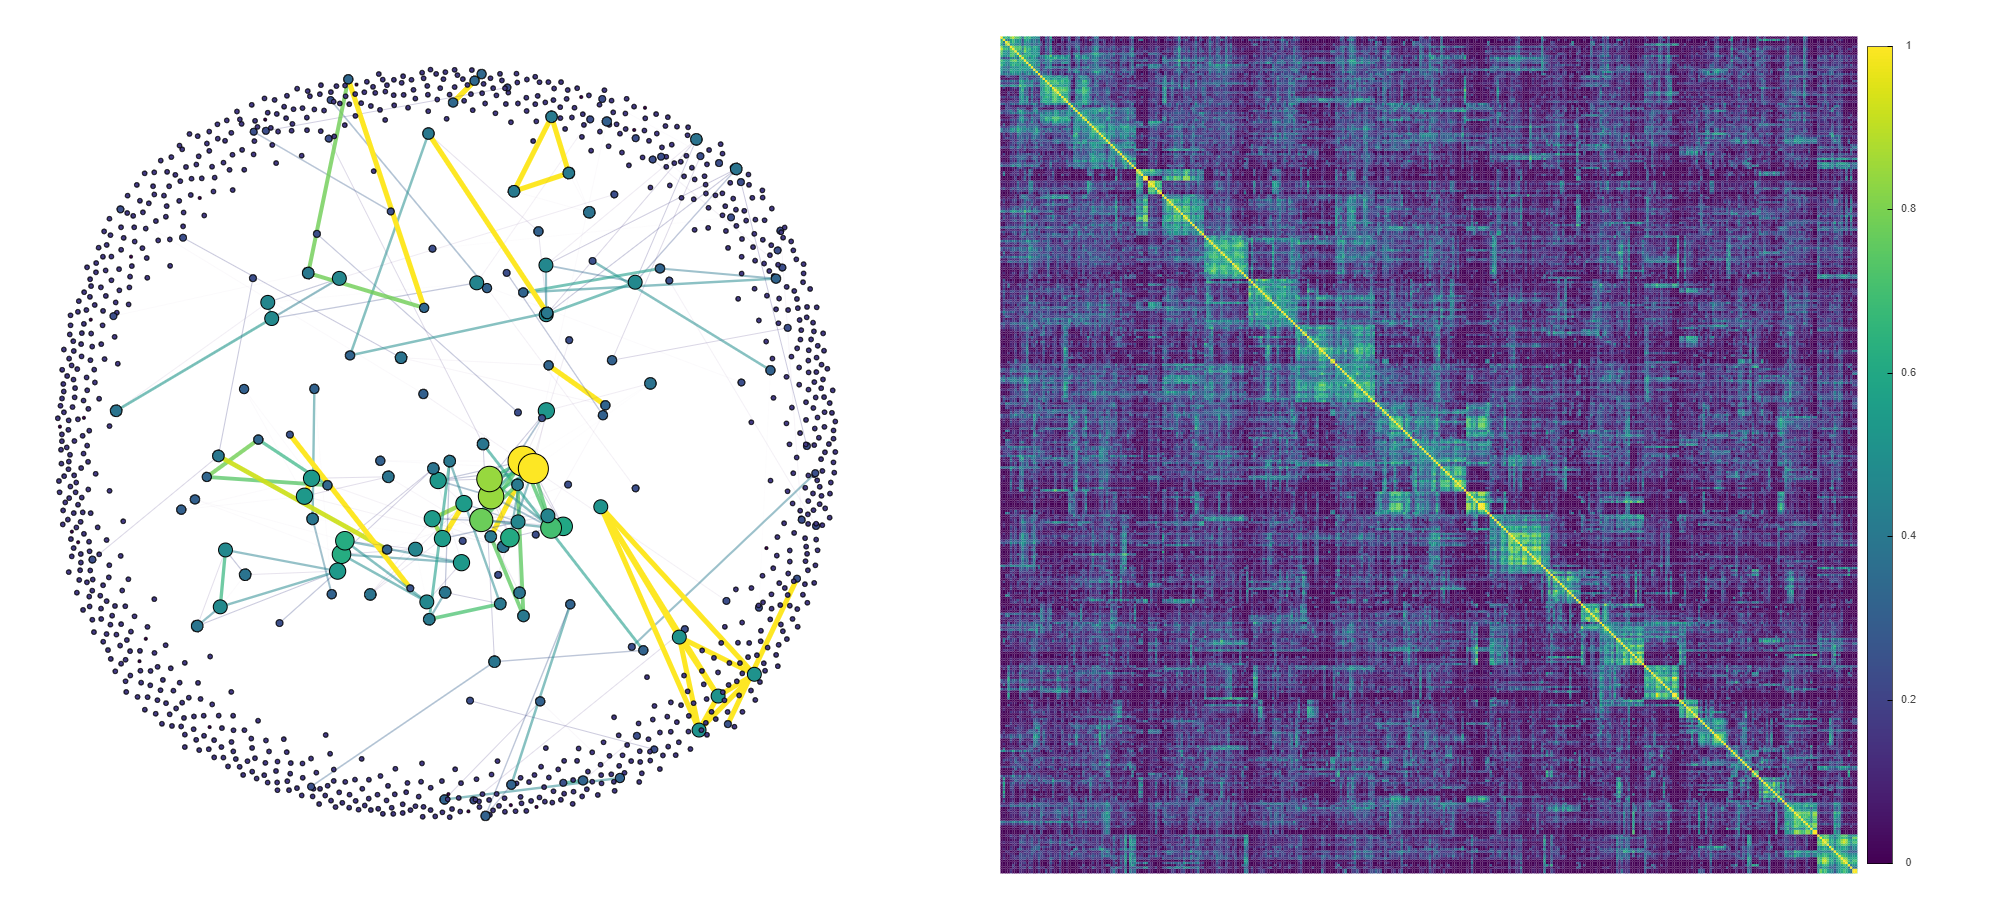
\includegraphics[width=\linewidth]{teaser.png}
  \caption{Left: non-datashaded node-link diagram with the force-directed layout. Right: zoomed in on part of the adjacency matrix reordered with the ward linkage and euclidean metric options. Dataset: the GephiMatrix\_author\_similarity dataset, filtered on edge-weight within the interval $[0.8, 1]$. The color palette is Viridis.}
	\label{fig:teaser}
}

%% Uncomment below to disable the manuscript note
\renewcommand{\manuscriptnotetxt}{}

%% Copyright space is enabled by default as required by guidelines.
%% It is disabled by the 'review' option or via the following command:
%\nocopyrightspace

%This command apparently has no use - Sam \vgtcinsertpkg

%%%%%%%%%%%%%%%%%%%%%%%%%%%%%%%%%%%%%%%%%%%%%%%%%%%%%%%%%%%%%%%%
%%%%%%%%%%%%%%%%%%%%%% START OF THE PAPER %%%%%%%%%%%%%%%%%%%%%%
%%%%%%%%%%%%%%%%%%%%%%%%%%%%%%%%%%%%%%%%%%%%%%%%%%%%%%%%%%%%%%%%%

\begin{document}

%% The ``\maketitle'' command must be the first command after the
%% ``\begin{document}'' command. It prepares and prints the title block.

%% the only exception to this rule is the \firstsection command
\firstsection{Introduction}

\maketitle

%% \section{Introduction} %for journal use above \firstsection{..} instead
% Tim van de Klundert and Sam Baggen
Humans are not inherently gifted at reading and interpreting large datasets, we are completely baffled upon viewing pages that are filled with numbers and text. But when those numbers are presented in forms of colorful graphs, everything is suddenly much clearer and easier to read, according to a study conducted by Vogel et al. \cite{Vogel:1986}. That is because the human eye is simply not that good at reading text and numbers. Luckily, computers are much better suited for this task as they can easily process hundreds of pages within a second.

Data visualizations combine the power of human intelligence and computer data processing power to analyze large amounts of data, which makes them very powerful. Since substantial amounts of data are readily available nowadays, visualization tools are required to find any insights in the data forest.
Our application is such a tool. It can both show an overview of the entire dataset and focus on specific subsets of the data.

% Sam Baggen
According to Okoe et al. \cite{Okoe:2018} the two most popular ways to visualize a graph are via a node-link diagram and an adjacency matrix. The reason for implementing both, a node-link diagram and an adjacency matrix, is because they have different advantages. Node-link diagrams are very useful for path-related tasks, as they outperform adjacency matrices to solve path-related tasks except for very large graphs as is shown in a study by Ghonheim et al. \cite{Ghonheim:2004}. In that same study, Ghonheim et al. also showed that adjacency matrices are more useful for finding specific nodes and specific links in comparison to node-link diagrams. However, more visualizations exist, such as 3D node-link diagrams.

\section{Related Work} % Sam Baggen
Our tool builds upon graph theory, as described in various books and articles by Matou\v{s}ek and Ne\v{s}et\v{r}il \cite{Matousek:2009}, Bollob\'{a}s \cite{Bollobas:1998}, Cormen et al \cite{Cormen:2009}, Diestel \cite{Diestel:2017} and many more. Furthermore, to enable the user to gain insights into the data that is visualized, at least one interaction from each category of interaction as defined in the paper by Yi et. al. \cite{Yi:2007} has been implemented. Additionally, to generate the node-link diagram layouts based on the algorithms described by Fruchterman and Reingold \cite{Fruchterman:1991}, and Gansner et al. \cite{Gansner:1993} several library functions were used. Lastly, various reordering techniques as described by Vogel et al. \cite{Vogel:1986}, Cohen-addad et al. \cite{Cohen-addad:2019:HCO:3338848.3321386}, Mello and Buzas \cite{mello1968application}, Glover \cite{DBLP:journals/corr/Glover16}, and Murtagh and Legendre \cite{DBLP:journals/corr/abs-1111-6285} are used.

\section{Technical Specifications} \label{sec:tech_spec}% Sam Baggen
In order to build the tool, it was decided to use Python and the PyViz environment. In particular, the packages Bokeh, Panel, HoloViews, NetworkX, Plotly, Pandas, Flask, and Nginx were predominantly used. Bokeh, NetworkX, Plotly, and HoloViews provide the visualizations. Panel is the library that enables us to have a multi-view system and makes the matrix reorderings possible. Pandas provides an easy way to manipulate and store data while Flask and Nginx provide support for running Python code in an online environment. These packages were chosen because HoloViews, which is an interface for Bokeh, seemed better than other packages for its simplicity for rendering graphs and providing native support for several types of interactions, like panning and zooming. Furthermore, HoloViews has native support for NetworkX which makes it easier to read data and convert it into a directed graph, something that was more complicated whilst only using Bokeh. Additionally, Pandas is used for data processing as all team members have previous experience with this package and it is an easy way to store and manipulate tabular data. The data that is accepted by our tool is in the format of an adjacency matrix and since it is tabular it matches perfectly with Pandas. Our back-end, which is all Python code, uses Bokeh, NetworkX, and Plotly to serve the graphs based on the data stored in Pandas. Then HoloViews instructs Bokeh to generate the appropriate JavaScript code which in turn is pushed to and executed on the client.

The front-end (the website) itself is written in HTML, CSS and JavaScript. The website has a homepage, where the user can get to know the people behind the tool, read this very report and watch an informative video about the tool and the team. On the homepage, a launch button is present to redirect the user to the tool. The users land on the file selection page where they can either select pre-uploaded datasets or upload their own dataset. When the user chooses a dataset, they will be redirected to the pre-filtering page. Here the user can apply constraints to the data which is used by the visualizations. After applying a filter, the user gets redirected to the page on which the visualizations are shown. The back-end processes the data and generates the visualizations, which are pushed to the client as soon as they are ready.

Whilst the user is waiting for the back-end to generate the visualizations, the page displays a loading screen to indicate that the data for the visualizations is being generated. These loading screens are fully programmed in JavaScript and disappear whenever the back-end has finished generating the visualizations, which will then be displayed instead.

\section{Pre-processing} %Sam Baggen
Before the data can be used for our visualization tool, it needs to be transformed and filtered. The data is ready to be visualized once all of these steps have been completed.

\subsection{File Upload and Handling} % Tim van de Klundert and Sam Baggen
Uploading the dataset may seem like a trivial task for our tool, however, all of the data must be processed and adjusted for proper usage by NetworkX and Bokeh. Every file must be processed on upload and stored in such a way that it is easy for the data to be reused, without re-initiating data processing. The specific input formats help with that task, as our tool expects the dataset to be a comma-separated values (.CSV) file, containing graph data in the adjacency matrix representation or an edge list (.EDGES) containing a list of pairs between nodes. Whether this graph is weighted, unweighted, directed, or undirected does not matter and gets detected automatically.

Upon uploading a file, it is sent to the back-end. In the back-end, basic checks will take place to make sure the file can actually be processed. These basic checks include a \textit{file format} check and a \textit{file integrity} check. The file format checks whether the uploaded file is a CSV, or EDGE file. The file integrity check will verify that the whole file has been submitted and that it has not been cut off due to a timeout. If the file passes these basic checks, it will be taken through the rest of the data processing. If the file fails one of the basic checks however, the user is taken back to the selection page. However, supplying the graph in the wrong representation will prove to be detrimental to our tool. This is because our tool currently assumes all parsed data to be in this representation and it is \textit{not} checked if that is the case.

After the uploading process has been completed, the back-end will read the file and convert it to a Pandas DataFrame. Due to how the data is supplied, the first column of the DataFrame would get the label "unnamed." To correct this, each subsequent column's label is shifted to the left such that the data in each column remains unchanged but the labels are in the correct spot again. Afterwards, the DataFrame is stored on the server in the HDF5 file format and is then subjected to filtering, as defined by the user, without modifying the stored dataset.
\subsection{Pre-filtering} \label{sect:prefiltering} % Sophia(Yuqing Zeng)
For the pre-filtering process, the user can choose between two methods, filtering by weight \& degree and filtering by clustering.% Steven van den Broek 
When the filtering by weight \&  degree method is chosen, distribution plots will be generated for assisting with the filtering. A kernel density estimate is used to generate this distribution. We chose this instead of a histogram to estimate the density, as the former is better at determining the shape of the distribution because they're not affected by the number of bins used and give an overall smoother result. We decided on using a Gaussian kernel for doing the density estimation. An important parameter for the kernel density estimation (KDE) is the bandwidth. To find a balance between performance and quality, we use Silverman's rule of thumb for getting a reasonable bandwidth with practically no increase in running time. The library KDEpy was chosen for doing the actual KDE since it outperforms all other, well-known, Python libraries.
% Sophia(Yuqing Zeng)

There will be a sequence of these distribution plots where one can select the range of allowed values. First the option to filter out edge-weights is given, and all edges that fall outside of the specified interval are removed. This filter is succeeded by a degree-based node filter, which first filters nodes by in-degree and then by out-degree. The user selects an interval that they deem appropriate for in-degree and out-degree, and only nodes with both in-degree and out-degree within the selected intervals shall be passed to the visualization tool.  

This three-layered weight and degree filtering method significantly reduces running time in the following section of the tool, while leaving users the freedom to customize which features of the dataset they wish to focus on. It also comes with a rather intuitive interface which will be further discussed in \ref{sect:pre-filter}.

The filtering process is optimized with sorting and binary-search algorithms so that it can process huge inputs (as large as a $10000\times 10000$ matrix) within a few seconds.When filtering edges based on weights, the DataFrame is first converted to a 1-D NumPy (a Python package) array that contains all edge-weights of the adjacency matrix. Then all entries of the 1-D array are sorted with an internal NumPy sorting method (QuickSort) and the original index reference is preserved for each entry. Thereafter, a binary-search is applied on the sorted array to locate the left and right cutoff points, and all entries with indices outside of the index range determined by the left and right cutoff points are reduced to 0. Lastly, with the index reference, the filtered entries are put back in their original order, and converted back to a DataFrame. The pseudocode for the aforementioned process excluding the conversion between DataFrame and NumPy matrix can be found in Algorithm \ref{alg:weight}. 

\begin{algorithm}[hbt]
\KwIn{n*n matrix $M_{in}$, int Left, int Right}
\KwOut{n*n matrix $M_{out}$}
  a $\leftarrow$ $Flatten$($M_{in}$); //Use NumPy.flatten, convert to a 1-D array\\
  a, index $\leftarrow$ $QuickSort$(a), $ArgSort$(a)\;
  l, r $\leftarrow$ $BinarySearch$(a, Left), $BinarySearch$(a, Right)\;
  b $\leftarrow$ [0]*a.length\; 
  j $\leftarrow$ l\;
 \While{j $<$ r}{
  i $\leftarrow$ index[j]\;
  b[i] $\leftarrow$ a[j]\;
  j $\leftarrow$ j + 1; }
 $M_{out} \leftarrow$ $Reshape$(b) \; 
 //Use NumPy.reshape, convert the array back to matrix \\
 \Return{$M_{out}$}
 \caption{Filter edges on weights}
 \label{alg:weight}
\end{algorithm}
Let $m$ denote the size (total elements) of the matrix. Run-time of this algorithm would be bounded by $O(m \, \text{log} \, m)$,  It employed both \textsc{QuickSort} and \textsc{BinarySearch} twice, which would be bounded by $O(m \, \text{log} \, m)$ and several iterations through elements in the matrix will take $O(m)$. 

% Edited by Tom Udding
When filtering nodes based on degree, a list of nodes to be removed is generated. 
For out-degree, each row is parsed and the remaining number of non-zero entries in that row are counted; for in-degree, each column parsed and the remaining number of non-zero entries in the column are counted. Once the degree of each row or column has been established, similar to the previous process, the degrees are sorted and put through a binary-search for the selected range. 
The pseudocode for the aforementioned process excluding the part of converting between the DataFrame and a NumPy matrix can be found in Algorithm \ref{alg:degree}.
%Yuqing Zeng
\begin{algorithm}[hbt]
\KwIn{n*n matrix $M_{in}$, int Left, int Right, Direction}
\KwOut{n*n matrix $M_{out}$}
 D $\leftarrow$ $emptyList$\; //Initialize the list of nodes to be deleted\\
 i $\leftarrow$ 0\;
 \eIf{Direction = $out$}{
   outDegree $\leftarrow$ $emptyList$\;
   \For{$i$ $<$ n}{
   row$\leftarrow$$M_{in}$[i]\;
   outDegree[i] $\leftarrow$ $countNonzero$(row)\;
   $i++$
   }
   l, r $\leftarrow$ $BinarySearch$(outDegree, Left), $BinarySearch$(outDegree, Right)\;
   D $\leftarrow$ outDegree[0: l] + outDegree[r:0 ]
   }{
   inDegree $\leftarrow$ $emptyList$\;
   \For{$i$ $<$ n}{
   col$\leftarrow Transpose(M_{in})$[i]\;
   inDegree[i] $\leftarrow$ $countNonzero$(col)\;
   $i++$
   }
   l, r $\leftarrow$ $BinarySearch$(inDegree, Left), $BinarySearch$(inDegree, Right)\;
    D $\leftarrow$ inDegree[: l] + inDegree[r: ]
  }
  $M_{in}$ $\leftarrow$ $DeleteRows(M_{in}, D)$\;
  $M_{out}$ $\leftarrow$ $DeleteColumns(M_{in}, D)$\;
 \Return{$M_{out}$}
 \caption{Filter nodes on degrees}
 \label{alg:degree}
\end{algorithm}
Let $m$ denote the size (total elements) of the matrix, and $n$ denote the width of the matrix. Run-time of this algorithm would be bounded by $O(n \, \text{log} \, n)$, since for each row/col it  calls \textsc{QuickSort} and \textsc{BinarySearch} twice, which would be bounded by $O(m \, \text{log} \, m)$ and several iterations through elements in the matrix will take $O(m)$. 

%Yuqin Cui
Unlike filtering by weights and degrees, which is applied to the whole dataset and returns the selected part of the dataset. Filtering by clustering splits a large dataset ($n \times n$) with more than 350 nodes into several small clusters mainly based on the $k$-means clustering algorithm.

Before performing $k$-means clustering on the whole dataset, a dimension reduction method called Principal Component Analysis (PCA)\cite{DBLP:reference/snam/2018} is applied to the original $n$-dimension dataset to compress it onto a 2-dimensional feature subspace with most of the relevant information preserved. This step is aiming to reduce the running time of the $k$-means algorithm by D. Arthur and S. Vassilvitskii \cite{DBLP:conf/compgeom/2006} from $O(n^{n\cdot k})$ to $O(n^{2 \cdot k })$, where $k = n/170 + 1$ is the number of clusters, determined by total number of nodes. After that, the original dataset is split based on its 2-dimensional feature with $k$-means algorithm\cite{DBLP:journals/sigpro/GalluccioMCH12} into $k$ of clusters. The information within each cluster is maintained and can be visualized later.

\subsection{Preparation for Visualization} %Sam Baggen
When the filtering process has been completed, the visualizations will be generated based on the filtered data. When the visualizations have been generated, the browser will receive the JavaScript code from the Bokeh server to draw the dataset. This JavaScript code allows callbacks to the Python code. Thus in the event that data is changed or needs to be changed (for instance when interacting with it), a Python callback is made to alter the visualization. The browser will then draw the newly generated data and allow the user to interact with it. What is drawn depends on the type of visualization the user has specified to be displayed.

\section{The Graphion Tool} % Sam Baggen
The tool itself is built out of four components: the website with all the information about the team, report, and video; dataset selection; data filtering (which is also referred to as pre-filtering); and the visualizations. Each component has its own section where it will be explained in more detail.

\subsection{The Website} \label{sect:website} % Sam Baggen
After the user has entered the URL into the address bar of the web browser, they will land on the homepage of the website. Here the user has the option to immediately launch the tool, which will redirect the user to the selection page, or to have a look at the report, video and the team. The report section features an abstract, and an image of the first page of the report. Underneath the abstract is a button to download the report. The team section contains portraits of all the team members, with their respective names underneath the portraits and their title. This title is not a serious title, but it represents to some extent the responsibilities of each team member. The video section of the page contains a button that will display the video.

\subsection{The Selection Page} % Sam Baggen
When the tool is launched, the user lands on the selection page. On this page, the user can choose whether to upload a dataset or pick a previously uploaded dataset. If the user wants to upload a dataset, they should press the ``Upload File''-button, after which they can choose between uploading an edge list or an adjacency matrix. Datasets can easily be dragged and dropped in order to be uploaded. If the user wants to pick a previously uploaded dataset, they should click on the ``Previously Uploaded''-button. Then a list of recently uploaded datasets is shown. If the user wants to use a previously uploaded dataset they should click on the name of the dataset. After uploading or choosing a dataset the user gets directed to the pre-filter page.

\begin{figure}[hbt]
    \centering
    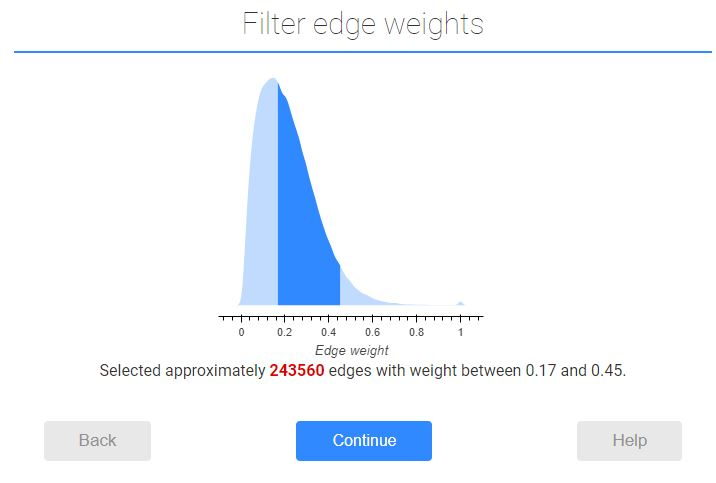
\includegraphics[width=0.45\textwidth]{Distplot.JPG}
    \caption{The user interface of the pre-filter page. This shows the edge distribution plot for the Gephimatrix\_author\_similarity dataset.}
    \label{fig:UISelect}
\end{figure}

\subsection{The Pre-Filter} \label{sect:pre-filter} % Sam Baggen, outdated no longer :)   
The pre-filter page shows the user an easy-to-use interface to filter out certain parts of the data in a dataset. There are four buttons present, the ``Interesting vertices / edges''-button, the ``Clusters''-button, the ``Help''-button, and the ``Back''-button. If the user is only interested in edges of a certain weight, and/or interested in vertices of a certain degree, then the user should click the ``Interesting vertices / edges''-button. After pressing the button, the user gets into a second menu where an interactive distribution plot is present, to help the user filter the data. Within this plot, the user defines an interval to which the edge-weight must adhere. Then the user specifies on a new distribution plot the interval to which the in-degree must adhere. After that a third distribution plot can be used to select the interval to which the out-degree must adhere. Underneath each plot a number is displayed that tells the user how many edges or vertices will be shown with the current selection, and the color of this number gives the user an indication of the time it takes to generate the visualizations. If the color is a shade of red, then the rendering process will take quite some time, if it is a shade of yellow it will take a medium amount of time and if it is a shade of green it will be done quite fast.

However, if the user is more interested in a cluster and wants to focus on that, then the user should press the ``Clusters''-button. The user then gets to see a plot with different sized circles on a diagonal line. Hovering over such a circle will tell the user the label of the cluster and how many nodes are in that cluster. Clicking on a cluster selects that cluster. When the user has configured the filter to be applied, the ``Continue''-button must be pressed to proceed to the final step. This step allows the user to specify whether datashading is enabled or not. By enabling datashading, edges are bundled using the DataShader package. When the user has ticked (or unticked) the checkbox the user must press the ``Start the tool''-button to start the filtering and rendering process, whereupon the user is redirected to the visualization page.

\subsection{The Visualization Page} \label{sect:vispage} %Sam Baggen
After having done the pre-filtering, the user ends up on this page. The visualizations page consists out of 2 major components: the GUI and the visualizations themselves. This section focuses on the GUI, whilst Section \ref{sect:Visualizations} will describe the visualizations themselves. The GUI, as seen in Figure \ref{fig:UI}, consists out of two toolbars: the left toolbar which contains the changeable parameters and the right toolbar which contains details about the selected edges and nodes. The left toolbar consists out of 10 elements, each with their own function. The right toolbar consists out of 2 elements, displaying different information. In the following list, each element is explained behind the number of the element. The labels can be found in Figure \ref{fig:UI}.

\begin{enumerate}
    \setlength\itemsep{0em}
    \item This link will take the user back to the homepage of the website as described in Section \ref{sect:website}.
    \item This link will take the user back through the pre-filtering process as described in Section \ref{sect:pre-filter}.
    \item These four buttons allow the user to switch between node-link diagram layouts. The available layouts are: force-directed (the default), radial, hierarchical, and 3D force-directed. More details about the node-link diagram can be found in Section \ref{sect:NL} and more information about the different layouts can be found in Section \ref{sect:NLlayouts}.
    \item This button can toggle the adjacency matrix on and off. By default it is shown, but clicking on it will hide the adjacency matrix. More details about the adjacency matrix can be found in Section \ref{sect:AM}.
    \item This dropdown allows the user to change the way of measuring distance. The available metrics are: eucledian, minkowski, cityblock, sqeuclidean, cosine, correlation, hamming, jaccard, chebyshev, canberra, and braycurtis. More information can be found towards the end of Section \ref{sect:AMreorderings}.
    \item The dropdown allows the user to reorder the adjacency matrix according to the various reordering algorithms. The available algortihms are: none, single, average, complete, centroid, weighted, median and ward. More details can be found in Section \ref{sect:AMreorderings}.
    \item This dropdown allows the user to resize the nodes based on a certain property of the nodes. By default, the size is determined by the in-degree of a node. The available properties are: in-degree, out-degree, total degree, total in edge weight, total out edge weight, and total edge weight.
    \item The dropdown allows the user to recolor the nodes based on a certain property of the nodes. By default, the color is determined by the total edge weight of a node. The available properties are: in-degree, out-degree, total degree, total in edge weight, total out edge weight, and total edge weight.
    \item The dropdown allows the user to change the color palette that the visualizations use. By default the "Black to Cyan" palette is used. The available palettes are: Black to Cyan, Green to Yellow, Blue to Green to Yellow, Blue to Violet to Pink, Blue to Magenta to Yellow, Cividis, Grayscale, Fire, Inferno, and Viridis.
    \item This switch enables and disables dark mode of the GUI respectively.
    \item This table shows information about the nodes in the node-link diagram and in the adjacency matrix. Selecting a node in the node-link diagram will highlight nodes here, highlight the connected edges in the table below, and highlight the relevant rows and columns in the adjacency matrix.
    \item This table shows information about the edges in the node-link diagram and the adjacency matrix. Selecting edges in the adjacency matrix will highlight the edges in this table, the relevant nodes in the table above, and the relevant nodes in the node-link diagram.
\end{enumerate}

\begin{figure*}[bt]
    \centering
    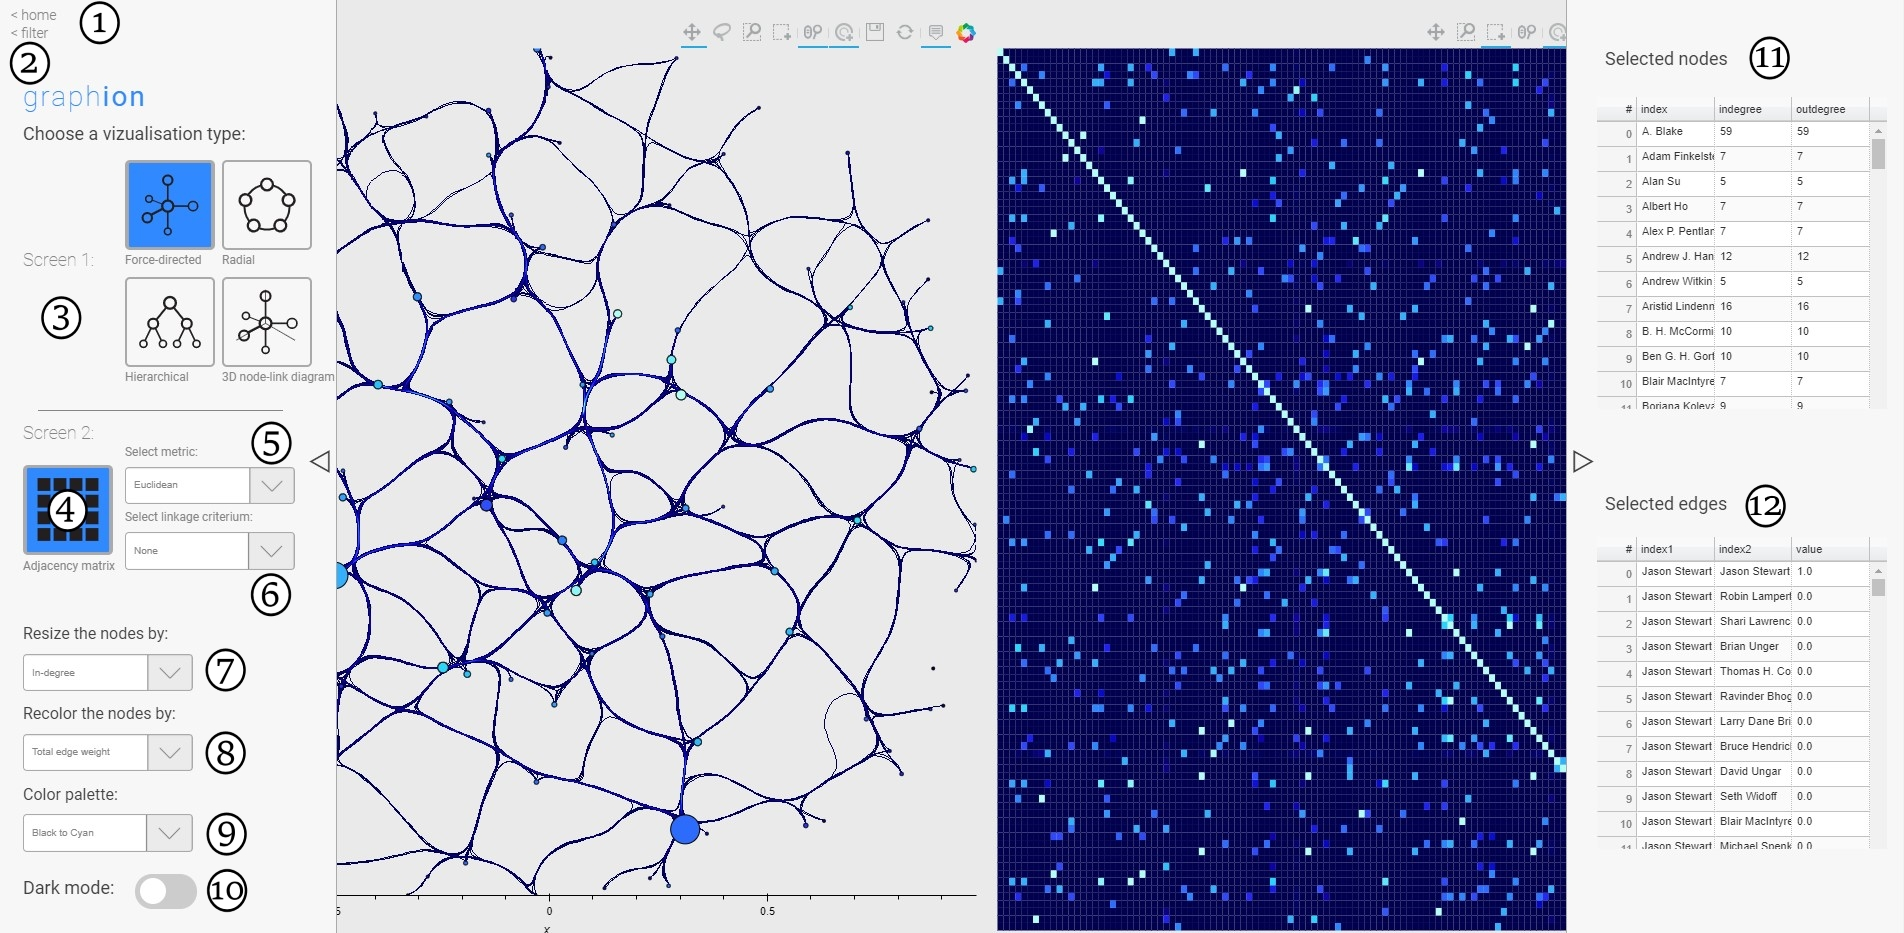
\includegraphics[width=0.95\textwidth]{GUI.jpg}
    \caption{The GUI of the Graphion tool. It consists out of a right toolbar with paramters and a left toolbar with information. The dataset shown in the background is the GephiMatrix\_author\_similarity dataset, pre-filtered with clustering, with cluster 1 selected.}
    \label{fig:UI}
\end{figure*}

\section{Visualizations} \label{sect:Visualizations} % Tim van de Klundert and altered by Sam Baggen
When the user enters the visualization page, an adjacency matrix will be shown on the right and a force-directed node-link diagram will be shown on the left. From this moment on, the user can start interacting with the dataset. These interactions include, but are not limited to: changing the node-link diagram layout, reordering the adjacency matrix, changing the color palette of both the adjacency matrix and the node-link diagram.

\subsection{Node-link Diagram} \label{sect:NL} % Sam Baggen
The node-link diagram is the most commonly used visual representation of a graph. It consists of a set of nodes, which are usually depicted by small circles or ovals and a set of links, denoted by lines. Links can only exist between two nodes and may either be directed or undirected. A graph can only contain one type of links and is thus as a whole directed or undirected. The links that are directed, are depicted by arrows where the arrowhead indicates the direction of the link. The layout and order of the nodes in a node-link diagram can differ quite a lot.

By default, the node-link diagram will use the force-directed layout. However, there are other layouts available, like radial or hierarchical. Furthermore, there is a 3-dimensional version of the force-directed layout available. Within the layouts, various things can be altered based on the properties of a node. The size and color of the nodes can be altered based on the in-degree, out-degree, total degree, weight of incoming edges, weight of outgoing edges, or total weight of in and outgoing edges. See Figure \ref{fig:NLExample} for an example of a force-directed node-link diagram of the GephiMatrix\_author\_similarity dataset.

\begin{figure}[hbt]
    \centering
    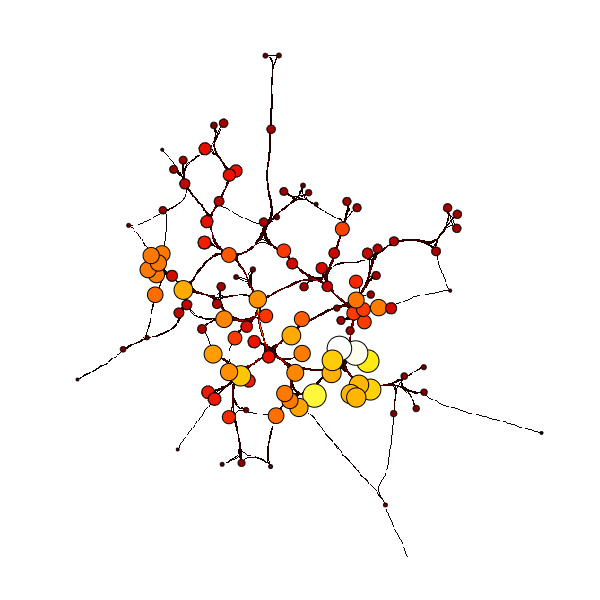
\includegraphics[width=0.3\textwidth]{example_nodelink.png}
    \caption{Example of a force-directed node-link diagram, using the clustering pre-filtering method choosing cluster 1 and having datashading enabled. The nodes are sized and colored based on total edge weight, using the Fire color palette.}
    \label{fig:NLExample}
\end{figure}

\subsection{Node-link Diagram Layouts} \label{sect:NLlayouts} %Sam Baggen
The tool supports three different layouts of the node-link diagram. 
\begin{enumerate}
    \setlength\itemsep{0em}
    \item Force-directed layout, using the Fruchterman-Reingold algorithm
    \item Radial layout
    \item Hierarchical layout
\end{enumerate}
In addition to these layouts, we also ahve a 3-dimensional version of the force-directed layout available.

\subsubsection{Force-Directed Layout}
The force-directed layout uses the Fruchterman-Reingold algorithm to determine the node positions \cite{Fruchterman:1991}. the goal of the layout is to create an aesthetically pleasing layout with as few link-crossings as possible.

\subsubsection{Radial Layout}
The radial layout will put all nodes on a circle, the unit circle to be exact. The clarity of the graph is determined by the user. If the user has enabled datashading in the pre-filter menu, then the edges are bundled and the user can distinguish individual edges more easily. However, if datashading is disabled then the edges will not be bundled and will become a solid circle if more than 2.500 edges are drawn. The user can no longer distinguish individual edges, which can be solved by zooming in on the diagram or by going back to the pre-filtering menu and enabling datashading (and hence also edge bundling).

\subsubsection{Hierarchical Layout}
The hierarchical layout will put nodes on horizontal lines, which themselves are stacked on top of each other to create a hierarchy, in such a way that the main flow or direction of the graph is shown. Based on the main orientation of edges, nodes are divided over the different lines to create a hierarchy of nodes. When following the edges, one should more often than not end up in the nodes that are in the bottom most line, 
giving the graph a top to bottom layout. This is done using a package called Graphviz, which uses the dot algorithm \cite{Gansner:1993}.

\subsection{Adjacency Matrix} \label{sect:AM} %Tim van de Klundert
The adjacency matrix is another powerful visualization to analyze data. An adjacency matrix is a matrix (or table in simple words), where each slot in the matrix is a number that denotes how strong the relationship (if any) between two nodes is. Then all numbers in the slots are mapped to colors (in our case, black for low numbers and blue for high numbers by default). This way, the matrix/table is basically translated to an image where each slot (which can become as small as a pixel for large datasets) displays a number in the original matrix. Figure \ref{fig:AMExample} shows an example of an adjacency matrix, of the GephiMatrix\_author\_similarity dataset.

\begin{figure}[hbt]
    \centering
    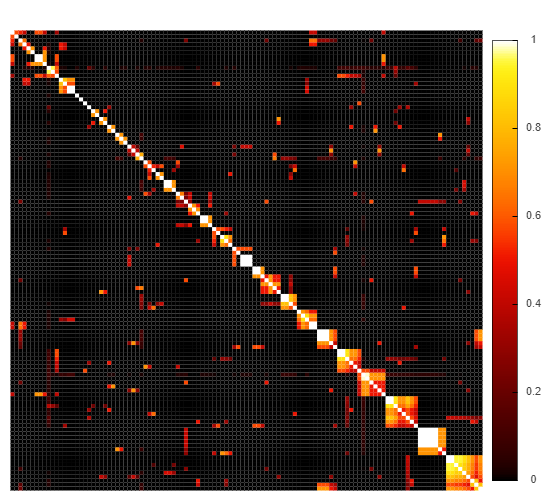
\includegraphics[width=0.38\textwidth]{example_matrix.png}
    \caption{Example of an adjacency matrix, using the clustering pre-filtering method choosing cluster 1 and having datashading enabled. The reordering method used is Ward, and the color palette is Fire.}
    \label{fig:AMExample}
\end{figure}

Notice that the adjacency matrix above has already been ordered before it was drawn. Due to the ordering, the color of a slot is often somewhat similar to the color of its neighboring slots. If it would not have been ordered, slots would often have random colors and the plot would be very hard to read. That is why finding a proper order for the rows and columns composing a visual matrix is essential for understanding datasets. Our tool automatically orders the adjacency matrix before it is shown, but the original order can be viewed by picking the None reordering.

The tool uses 7 reordering methods with different ways of calculating the similarity between two clusters in various distance metrics. There is also the possibility to use the original order of the dataset instead of using an ordering algorithm.

\subsection{Matrix reordering Algorithms} \label{sect:AMreorderings} % Yuqin Cui
All of the adjacency matrix reorderings are based on the hierarchical tree. The algorithm used is provided by the Python package \textit{fast-clustering}\cite{fastercluster}. Since the input dataset is a directed weighted graph, the adjacency matrix would be either symmetric or asymmetric, but always with $n \times n$ size, where $n$ is the number of vertices of the graph. 
The general procedure of our method works in three main steps\cite{DBLP:journals/cgf/BehrischBRSF16}:
\begin{itemize}
    \setlength\itemsep{0em}
    \item Generate a symmetric distance matrix based on the dataset the user uploaded.
    \item Calculate a hierarchical tree with hierarchical cluster analysis using different clustering methods, provided by the fast-clustering package.
    \item With the obtained hierarchical tree, traverse all the vertices from root to leaves. 
\end{itemize}
The agglomerative clustering method applied on an adjacency matrix and can be summarized as follows:

First, each node is treated as a single cluster, i.e., there are $n$ clusters for $n$ inputs nodes. Then, among all pairwise weight edges, a pair of nodes with shortest distance is clustered together and converted to a new node while removing themselves from graph. After that, $n-1$ nodes are left, and the distance from the new generated node to all the other nodes are determined by 7 methods \cite{fastercluster} which are listed below. The whole procedure would be repeated $n - 1$ times until all nodes are clustered into a single node. 

\begin{figure}[htbp]
  \centering
  \includesvg[width=0.35\textwidth]{Agg_cluster}
  \caption{Agglomerative clustering method: from single nodes to a whole cluster}
\end{figure}

\begin{itemize}
    \setlength\itemsep{0em}
    \item Single\cite{DBLP:conf/issnip/2013}: The minimum distance between any nodes in two clusters
    \item Complete\cite{DBLP:conf/mfcs/1997}: The maximum distance between any nodes in two clusters
    \item Average\cite{Cohen-addad:2019:HCO:3338848.3321386}: The average of summation of distance between all nodes in two clusters.
    \item Weighted\cite{mello1968application}: The average of the two distances determined by previous clusters.
    \item Centroid\cite{DBLP:journals/corr/Glover16}: The distance between centroids or means of two clusters.
    \item Ward's Method\cite{DBLP:journals/corr/abs-1111-6285}: The ESS (Error Sum of Squares) of the new cluster after combination of previous two clusters.
    \item Median(Weighted Pair Group Method using Centroids)\cite{Cohen-addad:2019:HCO:3338848.3321386}: The distance between centroids including counting weights of two clusters
\end{itemize}
The first three methods are graphics-based since the new clusters are presented by previous clusters or original sample points. The last four methods are geometric-based because the distances of new clusters are determined by a center point of previous clusters.

There are some shortages of the single-link and complete-link\cite{althaus2014greedy} methods, which can be improved by the average-link method. For the single-link method, it is easy to end up with a long chain and it causes clusters to spread out due to its clustering mechanism: only two nodes in the whole graph need to be close enough to form a pair, all others are irrelevant. The complete-link suffers from "crowding", since it only considers the worst-case distance between clusters. In other words, the node can be closer to the nodes in other clusters than its own. Average-link, which avoids both chaining and crowding, may change with a monotone increasing transformation of dissimilarities. Although none of these three clustering methods are optimized, users can choose their preference according to their demands.

Besides the clustering methods, 11 different distance measures (metrics) are provided to users. The default option is set to \textit{Euclidean metric}, which measures the \textit{ordinary} distance (as the crow flies) between two points in the Euclidean space. In most cases, geometry-based'  clustering would use \textit{Euclidean metric}. Another commonly used metric is \textit{Cityblock metric}, computing the Manhattan distance between the points, normally applied in datasets as networks.\cite{DBLP:journals/corr/BoraG14a}

Out of these reorderings, users can choose all options that they like and the matrix will be reordered afterwards. The drop-down menu allows users to choose several different methods described above to rearrange their datasets. This way, users can try all ordering methods to find information or patterns they are looking for. Also, the user can move the matrix around, by dragging the matrix to a different place within the visualization and can zoom in and out with their scroll wheel, if the user has clicked on the appopriate buttons.

\section{Interactions} %Yuqing Zeng(Sophia) 
Aside from generating the visualizations to be viewed, users are able to interact with the visualizations to explore data patterns and gain incisive knowledge. Following the seven categories of interactions \cite{Yi:2007}, one or more interactions for each category has been designed and implemented in the tool.

\subsection{Abstract or Elaborate}
This allows the user to view visualization with more or less detail. \cite{Yi:2007} In our tool, this is embodied as zoom in/out functions. When ``box zoom"-button above the visualization windows is selected, the user can drag and select the area of visualization they want to zoom into; when ``wheel zoom"-button is selected, the user can move mouse wheel down/up to zoom in/out on the visualization. The ``reset"-button lets the user reset to the default view. 

\subsection{Explore and Select}
Explore interaction allows the user to explore different parts of the visualization.\cite{Yi:2007}  With the ``pan"-button[include figure here] located above the visualization window selected, the user can click and drag around the view. This is especially useful when the visualization is zoomed in. 

Select interaction lets the user select and marks things as interesting. \cite{Yi:2007} In our tool, this is incarnated as the highlight function. With the ``Lasso Select"-button located above the visualization selected, the user can then drag and create a lasso, and highlight the nodes/edges within the lasso, this also applies to adjacency matrix, in this case; similarly, with the ``Box Select"-button selected, the user can highlight nodes/ within the box. 
With the ``tap"-button selected, the user can tap on select and highlight a single node/matrix.  

\subsection{Encode and Reconfigure} 
Encode allows for different representations of visualizations.\cite{Yi:2007} Users can swap between adjacency matrix and node-link diagram, or choose to have both of them displayed at the same time. Users are also able to change the color palette of both the adjacency matrix and node-link diagram (illustrated in Section \ref{sect:vispage} item 9) and resize/recolor nodes in a node-link diagram based on variables like out-degree(illustrated in Section \ref{sect:vispage} items 7 and 8).   

Reconfigure allows for rearrangements of visualizations. This is different from encoding, as the rearrangement happens within the same presentation.  This includes drop-down menus for different matrix reordering, that allows the user to change the order of matrix-cells(specific implementation details are discussed in the previous Section \ref{sect:AMreorderings}); and four buttons that allow a user to click and switch between node-link diagram layouts. (specific implementation details are discussed in the previous Section \ref{sect:NLlayouts}). 

\subsection{Filter}
This allows the user to decide what part of the data would be visualized through entering inputs. \cite{Yi:2007} 
Our filtering interaction is mainly implemented in the pre-filtering menu for pre-processing, this is further discussed in Section \ref{sect:pre-filter} and \ref{sect:prefiltering}.

\subsection{Connect}
This interaction allows the user to highlight related items in different visualizations. \cite{Yi:2007} In our tool, this is achieved by linking between node-link diagram and adjacency matrix. Highlighting edges in the matrix will highlight the nodes adjacent to these edges in the node-link diagram. Vice versa, selecting a node in the node-link will result in all the edges of that node, so a complete column and row, being highlighted. Moreover, information about the highlighted nodes/matrix cells will be visible on the right toolbar, the user can gain more insights from this information. 

The linking would only work under certain conditions. It is discussed in detail in Section \ref{sect:discussion}

\section{Back-end} % Tom Udding 
As previously described in section \ref{sec:tech_spec} the tool utilizes Python in combination with additional libraries, such as Bokeh, HoloViews, NetworkX, and Plotly, to provide the user-facing features and data, i.e. the visualizations. To get this data from Python to the user the tool runs on a Python-based Flask server using the Flask library. Embedded in this server is a Bokeh server. Flask is a micro web framework, meaning that it has all the essential tools to provide a minimal web server to be able to transfer data to and from the user. However, this is not practical in a real-world setup as our tool requires a more complex connection between the user and our visualization suite. Therefore, another library called Gunicorn is utilized. Gunicorn is a UNIX-based WSGI (Web Server Gateway Interface) for Python and allows us to use Bokeh to its full extent by providing callbacks through the embedded Bokeh server.
Because the tool is written as a Python module the tool can be easily embedded into existing systems. This modularity also allows for simple scalability of the tool since Nginx is utilised to proxy all connections to the Gunicorn server instance. Nginx can act as a load balancer to spread the load across multiple Flask instances but is by default configured to only use one Flask instance. This can easily be changed by modifying the existing code.
The server on which the tool is live is a cloud computing machine hosted by DigitalOcean in a data center located in Amsterdam. The specifications of the server are as follows; an Intel(R) Xeon(R) CPU E5-2650 v4 @ 2.20GHz processor (4 cores), 8GiB of RAM, a 160GiB SSD of which 64GiB is used as virtual memory to complement the 8GiB of RAM, and a dedicated 1GiB uplink and downlink for 40 USD (\$) per month.

\section{Application example} %Tim van de Klundert
To demonstrate how our tool works, the dataset GephiMatrix\_co-citation.csv (provided by the course) will be explored in our tool. The dataset is stored as an adjacency matrix in csv format and is undirected and sparse. This dataset gives for every pair of the 1053 authors an indication for the number of documents that cited both authors. Edges with a high weight indicate that the corresponding authors are often cited in the same document.

\subsection{Pre-filtering}
Once the user uploads the dataset, they can choose between filtering on edge weights and node degrees or focus on a cluster. For this demonstration, we will choose for clusters. Upon clicking on the ``Clusters''-button, a big and a small cluster become visible. We will pick the smaller one.
Since the cluster is not big, we can enable datashading without a need to wait multiple minutes to load the dataset. Once the loading is done, we can see the force-directed node-link diagram and the adjacency matrix in Figure \ref{fig:appexaample}.

\begin{figure}[hbt]
    \centering
    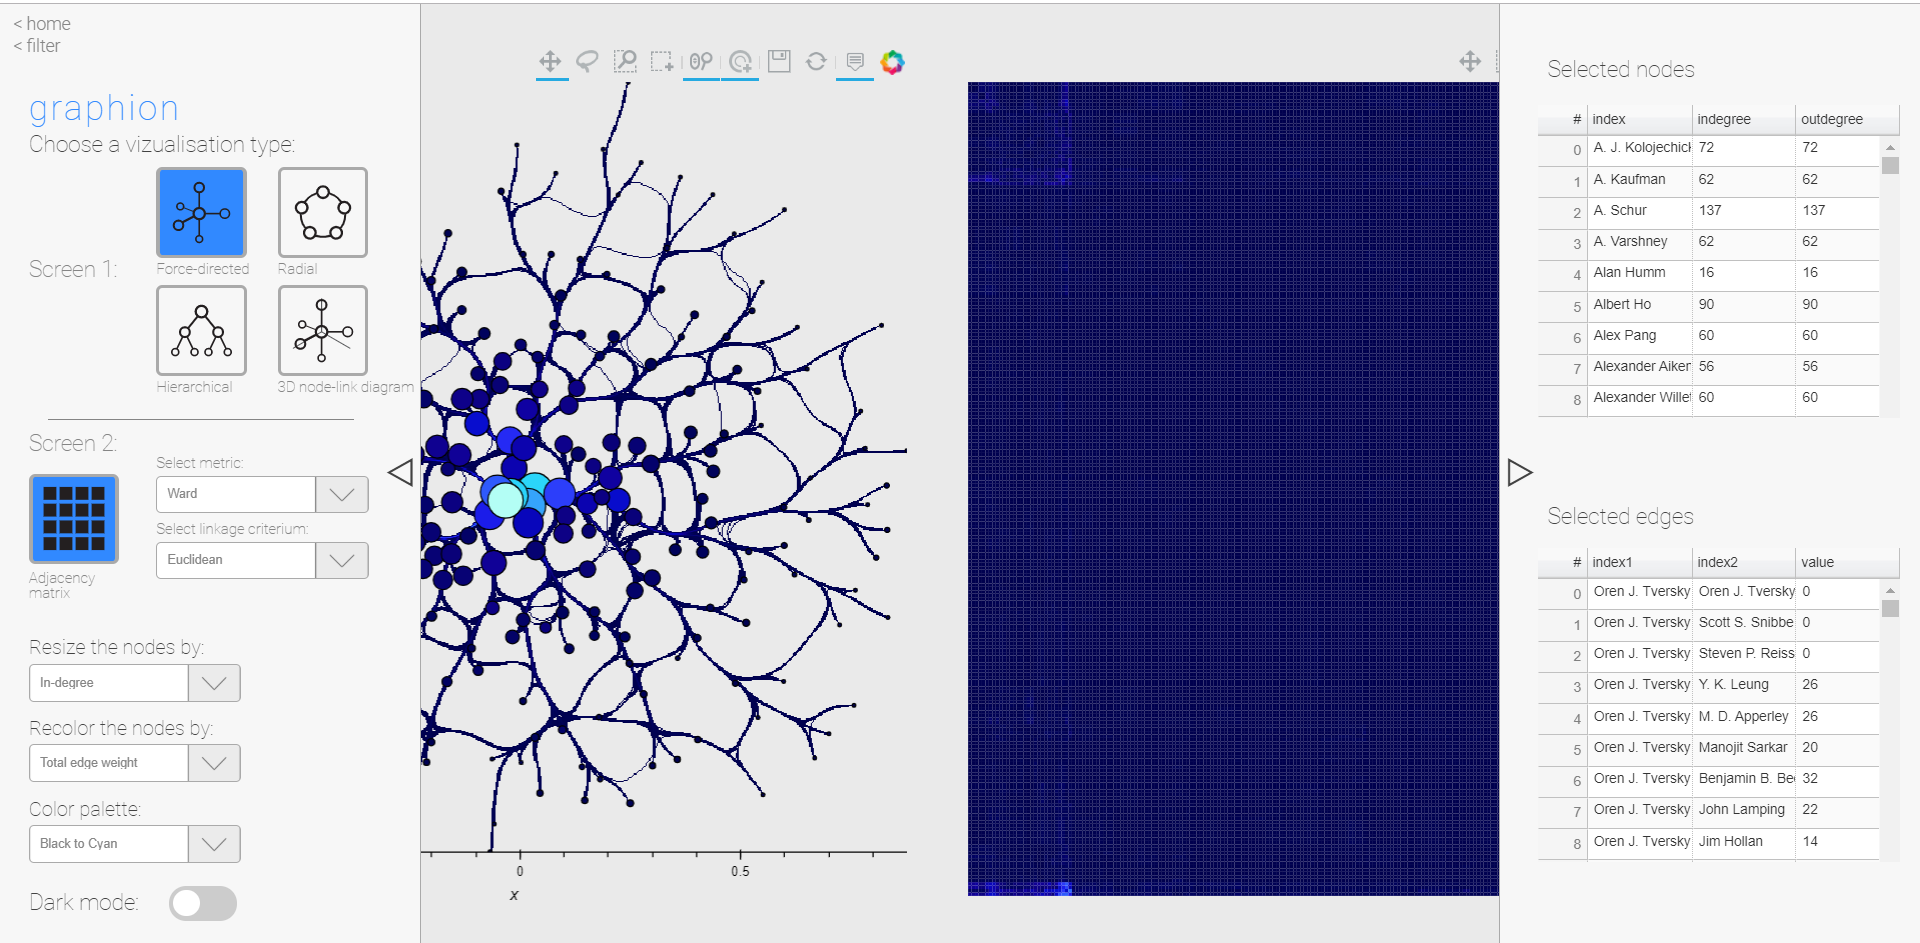
\includegraphics[width=0.5\textwidth]{app-example-1.png}
    \caption{The initial visualization of co-citation}
    \label{fig:appexaample}
\end{figure}

\subsection{Adjacency matrix}
The adjacency matrix has a few bright rectangles, but the one on the bottom right is clearly the brightest. The spots in those rectangles indicate that the two corresponding authors are often cited together in the same document. For instance, hovering over the two brightest spots in the bottom right of the matrix shows that Jock Mackinlay and Stuart Card are often cited together. There are two brightest spots because the dataset is symmetric. By hovering over the other spots in the bottom right corner it becomes clear that Jock Mackinlay, George R. Robertson, Ben Shneiderman and Stuart Card are often cited together.

\subsection{Node-link diagram}
The node-link diagram also looks interesting: There are a few big dots in the middle, the dots around the middle are somewhat smaller and the other nodes are all quite small. Big dots mean that the sum of the edge weights of edges connecting that dot is high, which indicates that the corresponding author is often cited together with other authors (or is just cited often). We will zoom in on the middle of the graph to take a closer look at the important nodes. Stuart Card has the biggest sum of edge weights of all writers in the chosen cluster. Jock Mackinlay and Ben Shneiderman also have a big sum of edge weights, but not as big as Stuart Card. George R. Robertson has the fourth biggest sum, but is not as popular as the other three. Ramana Rao is positioned in the center, but the sum of edge weights belongs more around the center. Notice that we encountered these names before in the adjacency matrix. When clicking on their dots, their places in the adjacency matrix will be highlighted. These authors appear to also have bright lines in the adjacency matrix, which makes perfect sense because they have many citations in total and thus should have more bright spots in the matrix.
% How shall I conclude this paragraph?

\section{Workflow} %Sophia(Yuqing) Zeng
We use two cloud platforms to update and synchronize our work. For all workflow-planning related documents (e.g. Peer Review Forms, Timesheets, Retrospectives, Agendas) we use  OneDrive, a free cloud storage tool developed by Microsoft. To keep all code synchronized, we use the version control platform GitHub. We also utilize its issue board function as a convenient online sprint board. Our team members will timely renew and resolve tasks on sprint boards, so even outside of meeting time, tasks can be efficiently generated from our backlog and distributed between the team members. Each person's working progress is also transparent to the whole team, which motivates task-completion and feedback communication, and ease the integration of individual codes into the main branch.

The workflow diagram in Figure \ref{fig:workflow} demonstrates how each component of our project relates to the others and in which sprint approximately it is developed.

\begin{figure}[hbt]
    \centering
    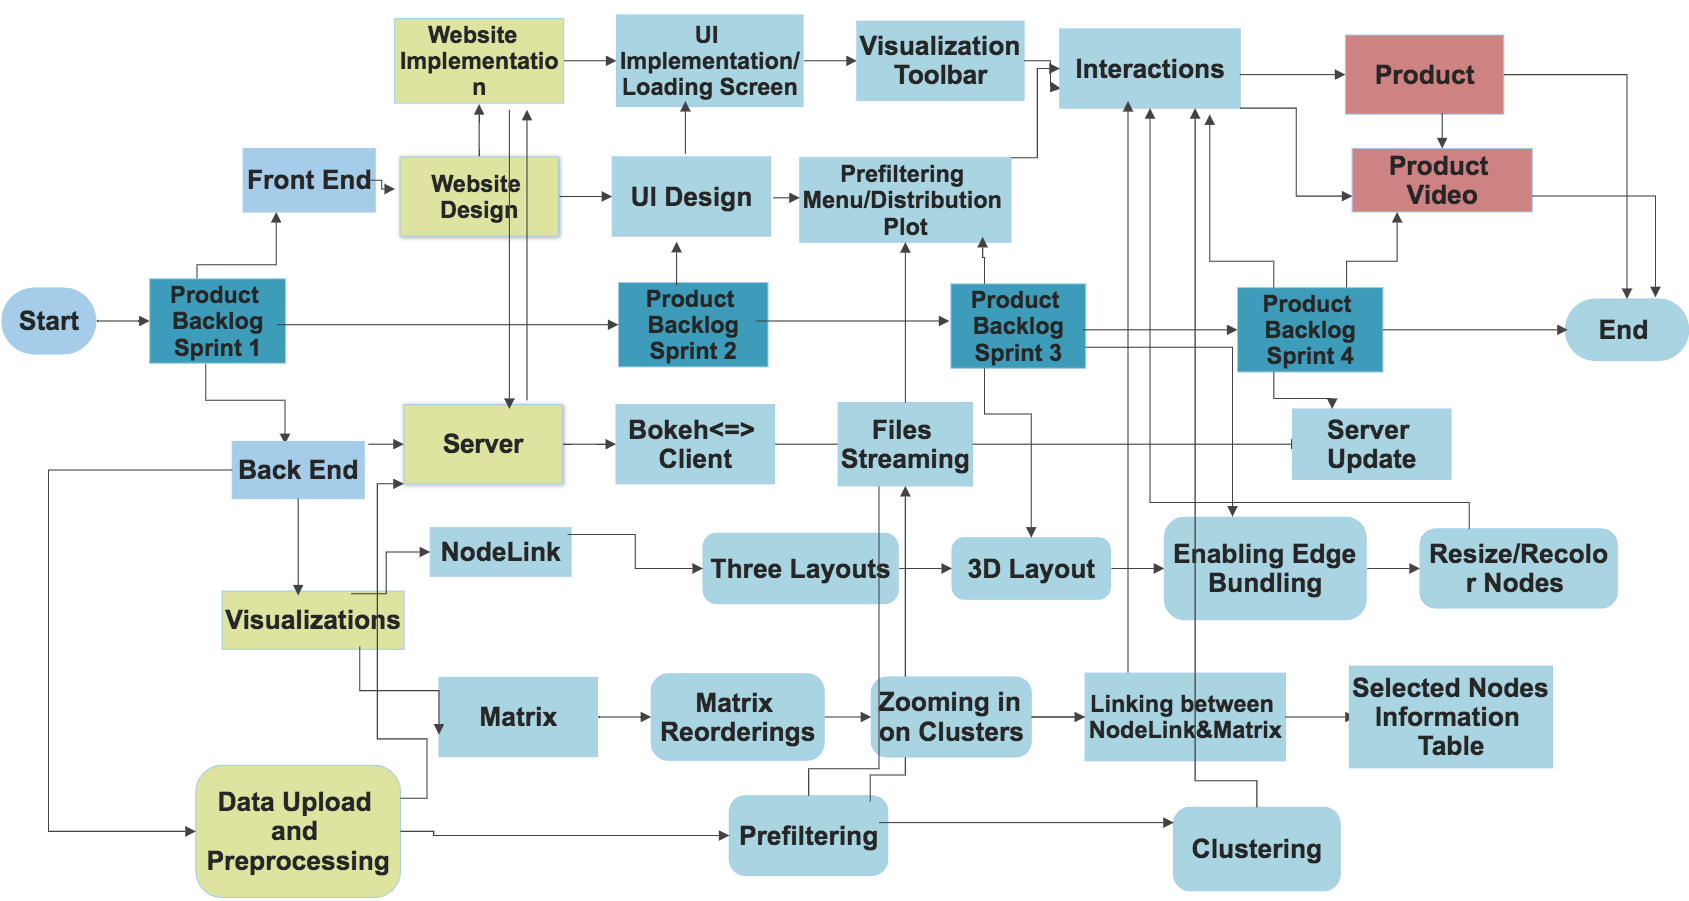
\includegraphics[width=0.5\textwidth]{Workflow.png}
    \caption{Workflow and Scrum Demonstration}
    \label{fig:workflow}
\end{figure}

\section{Discussion and limitations} \label{sect:discussion} %Tim van de Klundert and altered by Sam Baggen
During nine weeks of development, we managed to create a good visualization tool, but not a perfect one.
The tool excels at visualizing relatively small amounts of data. The strength of the adjacency matrix is the large number of available reordering combinations. Also, multiple color schemes can be chosen to see the differences more clearly and just for the beauty. Aside from that, the matrix is not so special, but an adjacency matrix is a quite simple concept, so it is hard to make a special one.
The node-link diagram is more interesting than the adjacency matrix. It supports 3 layouts: a radial layout, a hierarchical layout, a force-directed layout and it supports a 3-dimensional version of the force-directed layout. Thanks to the edge bundling of DataShader, the nodes are placed such that there will not be many edge crossings. Also, (parts of) edges will be combined if they can be close to each other. This all makes the node-link diagram very clear and easy to examine as well as just pretty to look at.

The main limitation of the tool is performance. The matrix will take a long time to load if there are many nodes and it will lose its responsiveness.
The node-link diagram is not able to handle a large number of edges. Due to the datashading that needs to take place before it can be visualized. This will take a very long time if there are many edges. According to the results of experimenting with the running time, edge bundling has a runtime complexity of about $O(E^2)$, where $E$ is the amount of edges, whereas the non-edge bundled version has a runtime complexity of about $O(E \cdot log(E))$. Also, it becomes less responsive if there are too many edges in the non-edge bundled version, but this effect will not occur quickly because our back-end will timeout if processing takes longer than 30 minutes.
Most of the performance problems described above are not in our direct control because we rely on libraries for many tasks, and some turned out to be quite slow. We managed to solve some performance problems, but not all of them.
As far as we know, the only way to solve these problems would be by starting over in another language, by using other libraries, or write more code from scratch.

To counteract the performance problems when visualizing large datasets, our tool has a powerful pre-filtering process that takes place before starting with visualizing. During pre-filtering, the user gets the opportunity to drop all edges that have a too small or too large weight and drop all nodes that have a too large or too small in-degree and out-degree. Alternatively, the pre-filtering can split the full dataset into clusters and the user can choose one of the clusters instead of the full dataset.
After the pre-filtering, only the data that was not filtered out will be visualized. If enough data was filtered out, our tool will work very well. For large datasets, the vast majority of the data will have to be filtered out. For small datasets, little or no data will need to be filtered out.
For very large datasets, the pre-filtering itself also has its limitations. The most important one is that it takes place on the back-end and thus the full dataset needs to be uploaded before the pre-filtering can start. Since moving data over the internet is not very fast, the uploading of very large datasets will take very long. Memory usage by unpacking and processing the uploaded datasets is also a limiting factor due to the nature of the space complexity of adjacency matrices.

Another limitation is the processing that is required for the pre-filtering. For very large datasets, this will take some time even with our optimized filtering process and also take a lot of memory. If the dataset is too large, the back-end could run out of memory, which makes it impossible no matter how patient the user is.
Probably the most frustrating limitation (to our team) is the linking between the node-link diagram and the adjacency matrix. As long as the visualizations are in their default setup, the linking works. However, as soon as something changes like applying an adjacency matrix reordering, changing the node-link diagram layout, or determining the node size by a different node property will break the linking. This is due to the Bokeh server generating a new JavaScript canvas that have the wrong linking events attached. This is done automatically by HoloViews (which instructs the Bokeh server) and thus is out of our control. The bug has been reported to the HoloViews GitHub repository \cite{Broek:2019}.

\section{Conclusion and Future Work} % Tim van de Klundert
This paper describes Graphion, a web-based visualization tool we have developed during the past nine weeks. It is an online visualization tool that allows users to upload and visualize datasets in the form of node-link diagrams and an adjacency matrix.
Just like any other tool, there is always room for improvement and new things that could be implemented.

% Tom Udding
Currently the tool has 3 distinct node-link diagrams, which provides the user with a lot of material. However, more types of node-link diagrams can be added, such as a spectral clustering node-link diagram as described by Shi and Malek \cite{shi2000normalized}.

Furthermore, the performance of the generation of the visualizations can be increased by tailoring the visualization algorithms based on the dataset. Currently the same algorithms are used for all datasets, however, for larger datasets more optimal and efficient algorithms exist, such as \textsc{sfdp} for force-directed node-link diagrams \cite{hu2005efficient}.

Even though HDF files and proper compression algorithms are used to reduce the storage footprint of uploaded datasets the required memory footprint of these datasets can be too big due to the space complexity of adjacency matrices. It would therefore be wise to implement an additional conversion process to convert the adjacency matrices to sparse matrices or edge lists.

Lastly, the tool will be complete when the linking between the node-link diagram and matrix can be implemented when the existing bug has been resolved \cite{Broek:2019}.

%Code below is not included in PDF but is here for BibTex instructions
\begin{comment}
\section{Bibliography Instructions}
\begin{itemize}
\item Sort all bibliographic entries alphabetically but the last name of the first author. This \LaTeX/bib\TeX\ template takes care of this sorting automatically.
\item Merge multiple references into one; e.\,g., use \cite{Max:1995:OMF,Kitware:2003} (not \cite{Kitware:2003}\cite{Max:1995:OMF}). Within each set of multiple references, the references should be sorted in ascending order. This \LaTeX/bib\TeX\ template takes care of both the merging and the sorting automatically.
\item Verify all data obtained from digital libraries, even ACM's DL and IEEE Xplore  etc.\ are sometimes wrong or incomplete.
\item Do not trust bibliographic data from other services such as Mendeley.com, Google Scholar, or similar; these are even more likely to be incorrect or incomplete.
\item Articles in journal---items to include:
  \begin{itemize}
  \item author names
	\item title
	\item journal name
	\item year
	\item volume
	\item number
	\item month of publication as variable name (i.\,e., \{jan\} for January, etc.; month ranges using \{jan \#\{/\}\# feb\} or \{jan \#\{-{}-\}\# feb\})
  \end{itemize}
\item use journal names in proper style: correct: ``IEEE Transactions on Visualization and Computer Graphics'', incorrect: ``Visualization and Computer Graphics, IEEE Transactions on''
\item Papers in proceedings---items to include:
  \begin{itemize}
  \item author names
	\item title
	\item abbreviated proceedings name: e.\,g., ``Proc.\textbackslash{} CONF\_ACRONYNM'' without the year; example: ``Proc.\textbackslash{} CHI'', ``Proc.\textbackslash{} 3DUI'', ``Proc.\textbackslash{} Eurographics'', ``Proc.\textbackslash{} EuroVis''
	\item year
	\item publisher
	\item town with country of publisher (the town can be abbreviated for well-known towns such as New York or Berlin)
  \end{itemize}
\item article/paper title convention: refrain from using curly brackets, except for acronyms/proper names/words following dashes/question marks etc.; example:
\begin{itemize}
	\item paper ``Marching Cubes: A High Resolution 3D Surface Construction Algorithm''
	\item should be entered as ``\{M\}arching \{C\}ubes: A High Resolution \{3D\} Surface Construction Algorithm'' or  ``\{M\}arching \{C\}ubes: A high resolution \{3D\} surface construction algorithm''
	\item will be typeset as ``Marching Cubes: A high resolution 3D surface construction algorithm''
\end{itemize}
\item for all entries
\begin{itemize}
	\item DOI can be entered in the DOI field as plain DOI number or as DOI URL; alternative: a URL in the URL field
	\item provide full page ranges AA-{}-BB
\end{itemize}
\item when citing references, do not use the reference as a sentence object; e.\,g., wrong: ``In \cite{Lorensen:1987:MCA} the authors describe \dots'', correct: ``Lorensen and Cline \cite{Lorensen:1987:MCA} describe \dots''
\end{itemize}
\end{comment}

%\section{Discussion and limitations}
%I think we should wait with this part until the end...

%\section{Conclusion}
%I think we should wait with this part until the end...

%% if specified like this the section will be committed in review mode
%\acknowledgments{
%The authors wish to thank A, B, and C. This work was supported in part by
%a grant from XYZ (\# 12345-67890).}

%\bibliographystyle{abbrv}
\bibliographystyle{abbrv-doi}
%\bibliographystyle{abbrv-doi-narrow}
%\bibliographystyle{abbrv-doi-hyperref}
%\bibliographystyle{abbrv-doi-hyperref-narrow}

\bibliography{template}
\end{document}

